\documentclass{article}

\usepackage{graphicx}
\usepackage{tikz}
\usepackage{tikzsymbols}
\usetikzlibrary{calc,patterns,shapes.geometric}
\pagestyle{empty}
\usepackage[margin=0pt]{geometry}
\geometry{papersize={14in,12in}}

\def\centerarc[#1](#2)(#3:#4:#5){\draw[#1] ($(#2)+({#5*cos(#3)},{#5*sin(#3)})$) arc (#3:#4:#5);}

\begin{document}
	\begin{figure}
		\centering
		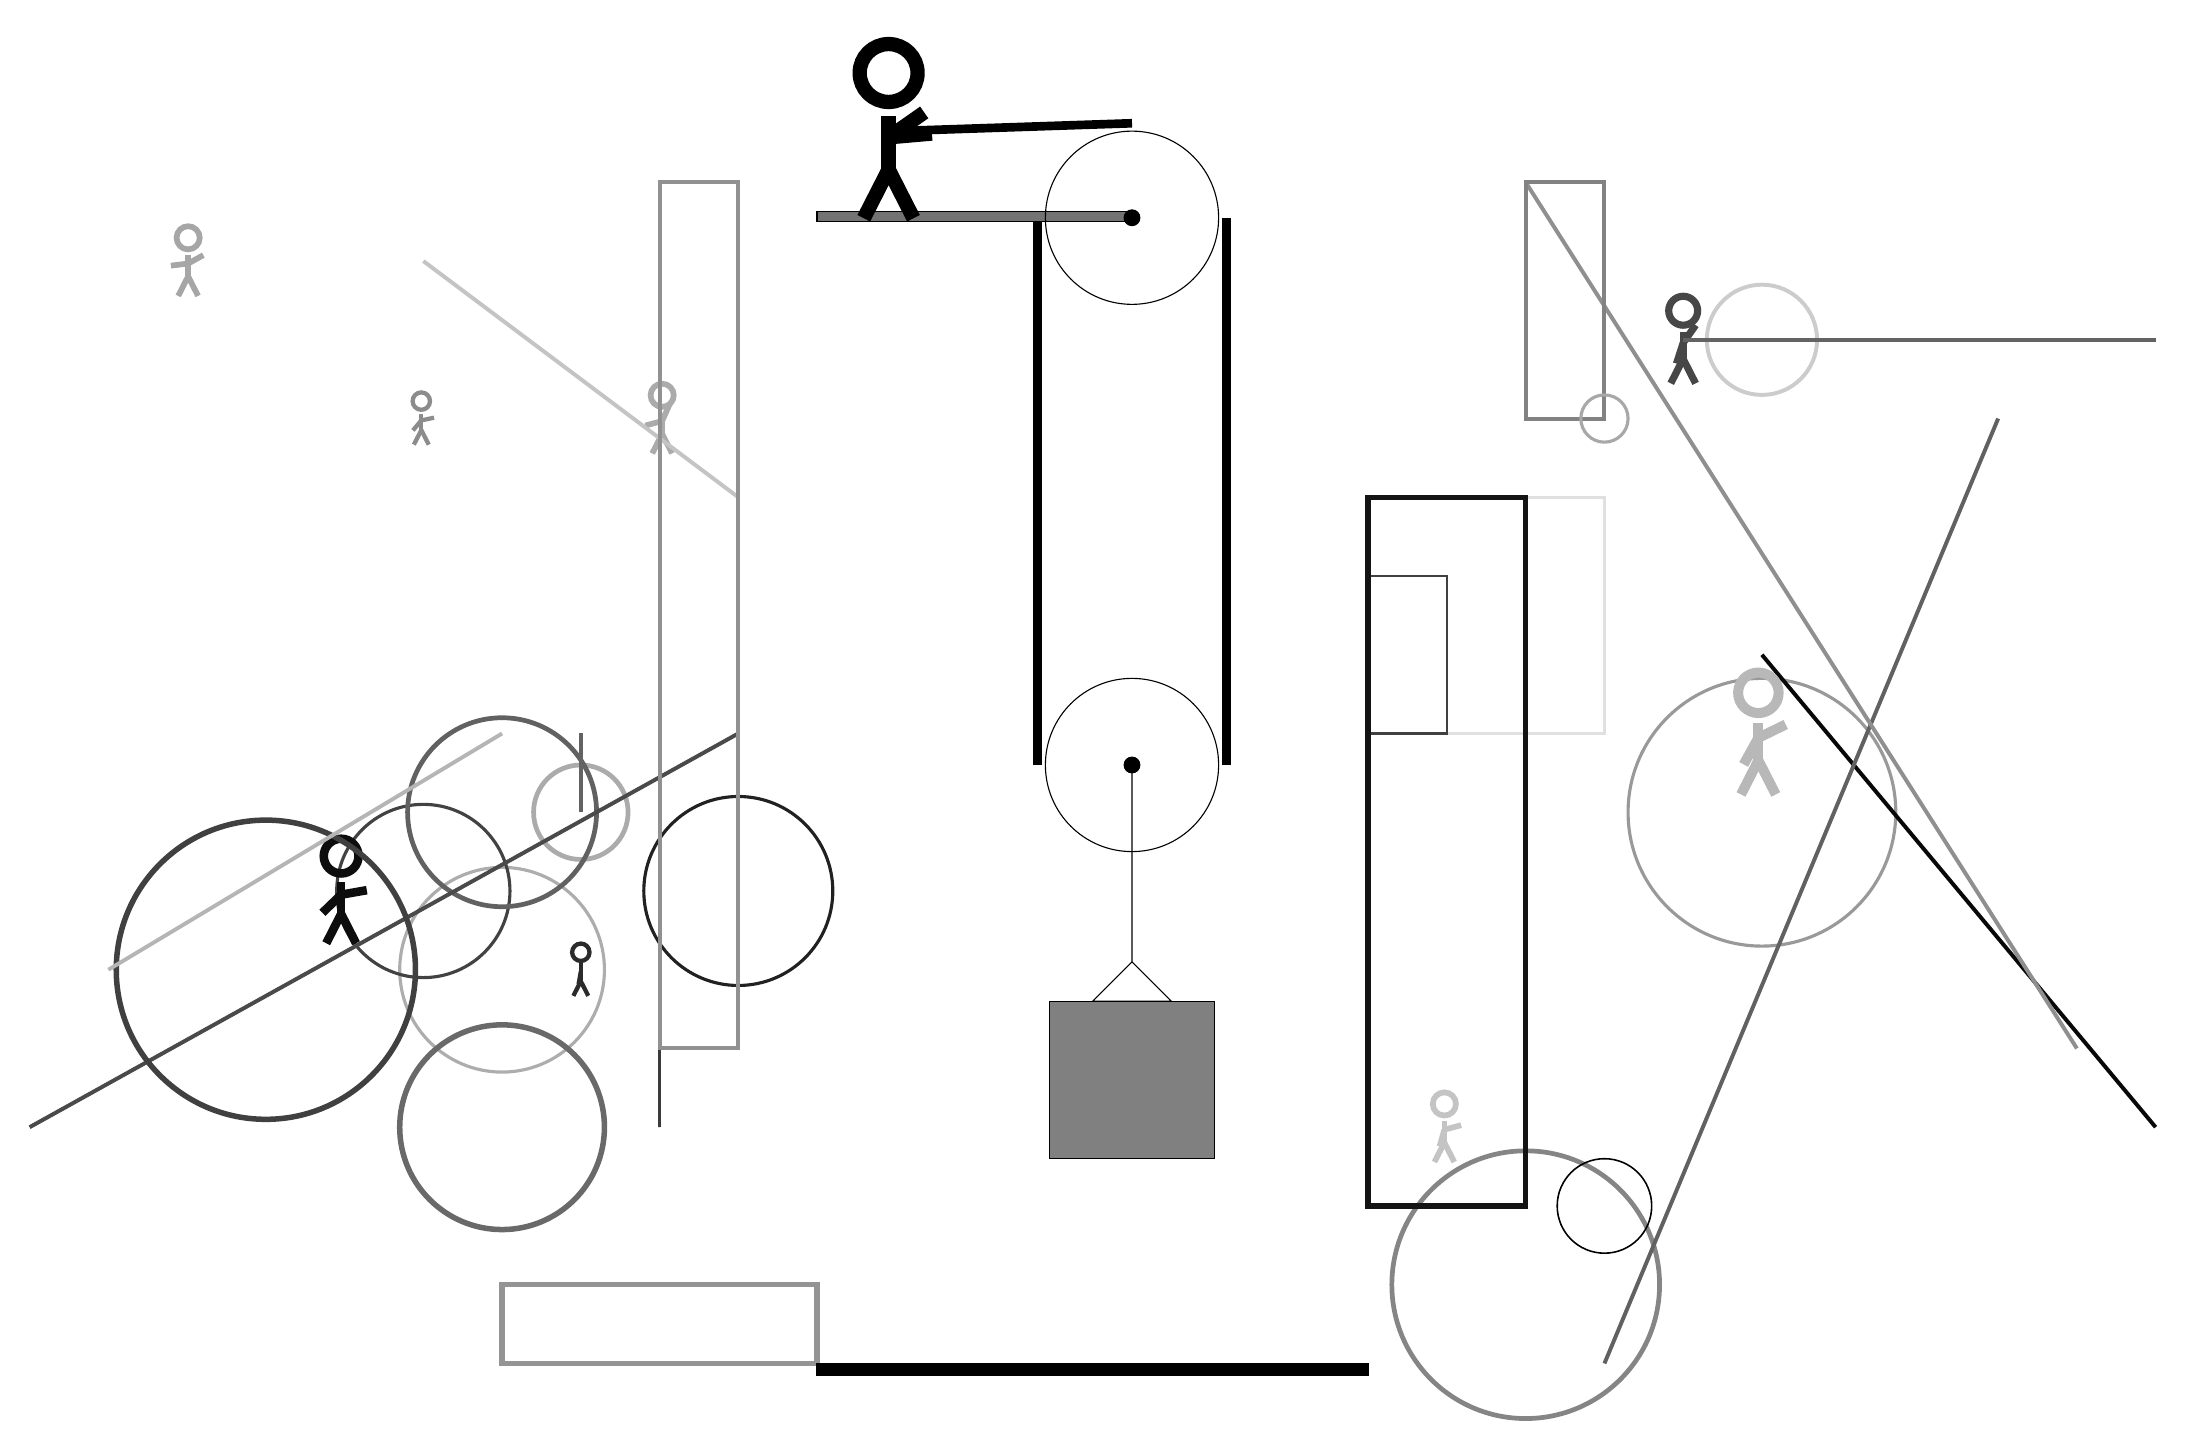
\begin{tikzpicture}
			%%%%% START %%%%%
			
			\draw[fill=black!55] (-2, 11.5) rectangle (2, 11.625);
			
			\draw (2, 4.6) circle (1.1);
			\draw[fill=black] (2, 4.6) circle (0.1);
			
			\draw (2, 11.55) circle (1.1);
			\draw[fill=black] (2, 11.55) circle (0.1);
			
			\draw (2, 4.6) -- (2, 2.1) -- (1.5, 1.6) -- (2.5, 1.6) -- (2, 2.1);
			\draw[fill=black!50] (0.95, 1.6) rectangle (3.05, -0.4);
			
			\draw[line width=1.1mm] (0.8, 11.5) -- (0.8, 4.6);
			\centerarc[line width=1.1mm](2, 4.6)(180:360:1.2000000000000002);
			\draw[line width=1.1mm](3.2, 4.6) -- (3.2, 11.55);
			\centerarc[line width=1.1mm](2, 11.55)(0:90:1.2000000000000002);
			\draw[line width=1.1mm](2, 12.75) -- (-1, 12.65);
			
			\node at (-1, 12.65) {\Strichmaxerl[10][-175][35]};
			
			\draw [line width=0.6mm, color=black!48](7, -2) circle (1.7);
			
			\draw[line width=0.4mm, color=black!12] (5, 5) rectangle (8, 8);
			\draw [line width=0.4mm, color=black!40](10, 4) circle (1.7);
			\node[line width=0.2mm, color=black!33] at (-4, 9) {\Strichmaxerl[4][15][66]};
			\draw[line width=0.3mm, color=black!75] (5, 7) rectangle (6, 5);
			
			\draw [line width=0.4mm, color=black!32](-6, 2) circle (1.3);
			\draw[line width=0.4mm, color=black!77] (-4, 0) rectangle (-4, 3);
			\draw [line width=0.6mm, color=black!33](-5, 4) circle (0.6);
			\draw [line width=0.4mm, color=black!87](-3, 3) circle (1.2);
			\draw [line width=0.4mm, color=black!74](-7, 3) circle (1.1);
			\draw [line width=0.5mm, color=black!20](10, 10) circle (0.7);
			
			\draw [line width=0.6mm, color=black!62](-6, 4) circle (1.2);
			\draw[line width=0.5mm, color=black!61](-5, 5) -- (-5, 4);
			\draw[line width=0.5mm, color=black!97](10, 6) -- (15, 0);
			\draw[line width=0.7mm, color=black!42] (-2, -2) rectangle (-6, -3);
			\node[line width=0.2mm, color=black!95] at (-8, 3) {\Strichmaxerl[6][44][10]};
			
			\node[line width=0.3mm, color=black!72] at (9, 10) {\Strichmaxerl[5][72][55]};
			
			\draw[line width=0.5mm, color=black!71](-3, 5) -- (-12, 0);
			\draw [line width=0.7mm, color=black!75](-9, 2) circle (1.9);
			
			\draw[line width=0.5mm, color=black!62](8, -3) -- (13, 9);
			\node[line width=0.6mm, color=black!45] at (-7, 9) {\Strichmaxerl[3][50][12]};
			\draw [line width=0.7mm, color=black!59](-6, 0) circle (1.3);
			\node[line width=0.4mm, color=black!35] at (-10, 11) {\Strichmaxerl[4][7][29]};
			\node[line width=0.3mm, color=black!83] at (-5, 2) {\Strichmaxerl[3][80][90]};
			\draw[line width=0.5mm, color=black!44](7, 12) -- (14, 1);
			
			\node[line width=0.4mm, color=black!28] at (10, 5) {\Strichmaxerl[7][61][26]};
			\draw[line width=0.7mm, color=black!92] (5, -1) rectangle (7, 8);
			\draw[line width=0.5mm, color=black!23](-3, 8) -- (-7, 11);
			\draw[line width=0.5mm, color=black!29](-6, 5) -- (-11, 2);
			\draw[line width=0.5mm, color=black!49] (7, 9) rectangle (8, 12);
			\draw [line width=0.2mm, color=black!100](8, -1) circle (0.6);
			
			\draw[line width=0.5mm, color=black!43] (-4, 12) rectangle (-3, 1);
			\draw[line width=0.5mm, color=black!61](9, 10) -- (15, 10);
			\node[line width=0.2mm, color=black!23] at (6, 0) {\Strichmaxerl[4][74][15]};
			\draw [line width=0.4mm, color=black!34](8, 9) circle (0.3);
			
			\draw[fill=black] (-2, -3) rectangle (5, -3.15);
			
			%%%%% END %%%%%
		\end{tikzpicture}
	\end{figure}	
\end{document}